\documentclass{article}

\usepackage{fancyhdr}
\usepackage{wrapfig}
\usepackage{extramarks}
\usepackage{multicol}
\usepackage{amsmath}
\usepackage{amsthm}
\usepackage{amsfonts}
\usepackage{tikz}
\usepackage[plain]{algorithm}
\usepackage{algpseudocode}
\usepackage{enumerate}
\usepackage[shortlabels]{enumitem}                                          
                    \setlist[enumerate, 1]{1\textsuperscript{o}}



\usepackage{listings}
\usepackage{xcolor}
\lstset { %
    language=C++,
    backgroundcolor=\color{black!5}, % set backgroundcolor
    basicstyle=\footnotesize,% basic font setting
}

%\usetikzlibrary{automata,positioning}
\usetikzlibrary{positioning,shapes,shadows,arrows,automata}

%
% Basic Document Settings
%

\topmargin=-0.45in
\evensidemargin=0in
\oddsidemargin=0in
\textwidth=6.5in
\textheight=9.0in
\headsep=0.25in

\linespread{1.1}

\pagestyle{fancy}
\lhead{\hmwkAuthorName}
\chead{\hmwkClass\ (\hmwkClassInstructor\ \hmwkClassTime): \hmwkTitle}
\rhead{\firstxmark}
\lfoot{\lastxmark}
\cfoot{\thepage}

\renewcommand\headrulewidth{0.4pt}
\renewcommand\footrulewidth{0.4pt}

\setlength\parindent{0pt}

%
% Create Problem Sections
%

\newcommand{\enterProblemHeader}[1]{
    \nobreak\extramarks{}{Problem \arabic{#1} continued on next page\ldots}\nobreak{}
    \nobreak\extramarks{Problem \arabic{#1} (continued)}{Problem \arabic{#1} continued on next page\ldots}\nobreak{}
}

\newcommand{\exitProblemHeader}[1]{
    \nobreak\extramarks{Problem \arabic{#1} (continued)}{Problem \arabic{#1} continued on next page\ldots}\nobreak{}
    \stepcounter{#1}
    \nobreak\extramarks{Problem \arabic{#1}}{}\nobreak{}
}

\setcounter{secnumdepth}{0}
\newcounter{partCounter}
\newcounter{homeworkProblemCounter}
\setcounter{homeworkProblemCounter}{1}
\nobreak\extramarks{Problem \arabic{homeworkProblemCounter}}{}\nobreak{}

%
% Homework Problem Environment
%
% This environment takes an optional argument. When given, it will adjust the
% problem counter. This is useful for when the problems given for your
% assignment aren't sequential. See the last 3 problems of this template for an
% example.
%
\newenvironment{homeworkProblem}[1][-1]{
    \ifnum#1>0
        \setcounter{homeworkProblemCounter}{#1}
    \fi
    \section{Problem \arabic{homeworkProblemCounter}}
    \setcounter{partCounter}{1}
    \enterProblemHeader{homeworkProblemCounter}
}{
    \exitProblemHeader{homeworkProblemCounter}
}

%
% Homework Details
%   - Title
%   - Due date
%   - Class
%   - Section/Time
%   - Instructor
%   - Author
%

\newcommand{\hmwkTitle}{Homework\ \#1}
\newcommand{\hmwkDueDate}{January 20 2015}
\newcommand{\hmwkClass}{CS581 Theory of Computation}
\newcommand{\hmwkClassTime}{Winter 2016}
\newcommand{\hmwkClassInstructor}{Harry H. Porter}
\newcommand{\hmwkAuthorName}{Konstantin Macarenco}

%
% Title Page
%

\title{
    \vspace{2in}
    \textmd{\textbf{\hmwkClass:\ \hmwkTitle}}\\
    \normalsize\vspace{0.1in}\small{Due\ on\ \hmwkDueDate\ at 2:00pm}\\
    \vspace{0.1in}\large{\textit{\hmwkClassInstructor\ \hmwkClassTime}}
    \vspace{3in}
}

\author{\textbf{\hmwkAuthorName}}
\date{}

\renewcommand{\part}[1]{\textbf{\large Part \Alph{partCounter}}\stepcounter{partCounter}\\}

%
% Various Helper Commands
%

% Useful for algorithms
\newcommand{\alg}[1]{\textsc{\bfseries \footnotesize #1}}

% For derivatives
\newcommand{\deriv}[1]{\frac{\mathrm{d}}{\mathrm{d}x} (#1)}

% For partial derivatives
\newcommand{\pderiv}[2]{\frac{\partial}{\partial #1} (#2)}

% Integral dx
\newcommand{\dx}{\mathrm{d}x}

% Alias for the Solution section header
\newcommand{\solution}{\textbf{\large Solution}}

% Probability commands: Expectation, Variance, Covariance, Bias
\newcommand{\E}{\mathrm{E}}
\newcommand{\Var}{\mathrm{Var}}
\newcommand{\Cov}{\mathrm{Cov}}
\newcommand{\Bias}{\mathrm{Bias}}

\begin{document}

\maketitle

\pagebreak

\begin{homeworkProblem}

\noindent

\begin{center}
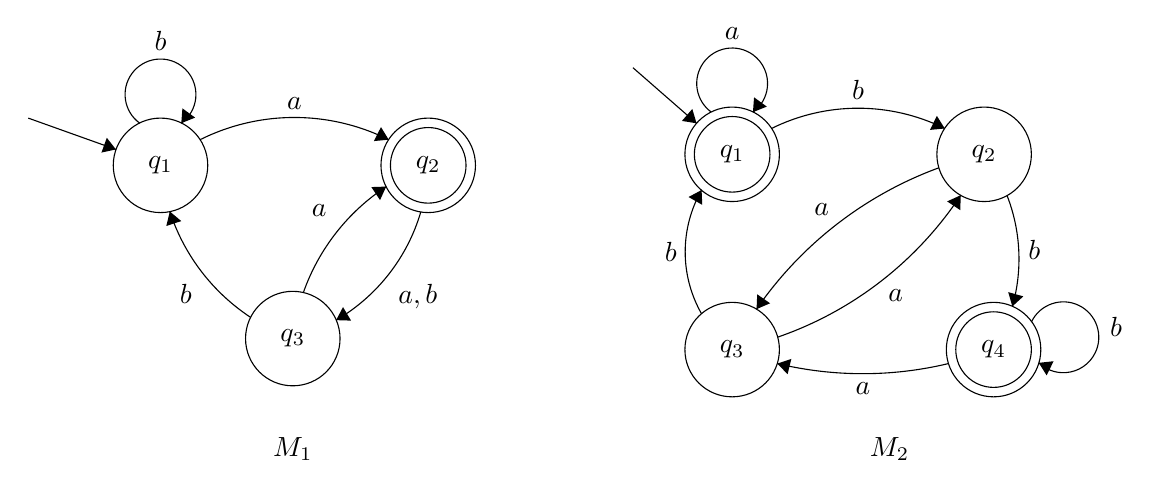
\begin{tikzpicture}[scale=0.2]
\tikzstyle{every node}+=[inner sep=0pt]
\draw [black] (9.8,-10.1) circle (3);
\draw (9.8,-10.1) node {$q_1$};
\draw [black] (26.8,-10.1) circle (3);
\draw (26.8,-10.1) node {$q_2$};
\draw [black] (26.8,-10.1) circle (2.4);
\draw [black] (18.2,-21.1) circle (3);
\draw (18.2,-21.1) node {$q_3$};
\draw (18.2,-28.1) node {$M_1$};
\draw [black] (46.1,-9.4) circle (3);
\draw (46.1,-9.4) node {$q_1$};
\draw [black] (46.1,-9.4) circle (2.4);
\draw [black] (62.1,-9.4) circle (3);
\draw (62.1,-9.4) node {$q_2$};
\draw [black] (46.1,-21.8) circle (3);
\draw (46.1,-21.8) node {$q_3$};
\draw (56.1,-28.1) node {$M_2$};
\draw [black] (62.7,-21.8) circle (3);
\draw (62.7,-21.8) node {$q_4$};
\draw [black] (62.7,-21.8) circle (2.4);
\draw [black] (8.477,-7.42) arc (234:-54:2.25);
\draw (9.8,-2.85) node [above] {$b$};
\fill [black] (11.12,-7.42) -- (12,-7.07) -- (11.19,-6.48);
\draw [black] (12.312,-8.472) arc (116.53845:63.46155:13.402);
\fill [black] (24.29,-8.47) -- (23.8,-7.67) -- (23.35,-8.56);
\draw (18.3,-6.56) node [above] {$a$};
\draw [black] (26.329,-13.055) arc (-16.32928:-59.70861:11.807);
\fill [black] (20.95,-19.93) -- (21.9,-19.96) -- (21.39,-19.1);
\draw (24.87,-18.42) node [right] {$a,b$};
\draw [black] (18.87,-18.182) arc (160.62375:123.33837:13.357);
\fill [black] (24.13,-11.45) -- (23.19,-11.48) -- (23.74,-12.31);
\draw (20.38,-12.97) node [left] {$a$};
\draw [black] (15.525,-19.756) arc (-123.37352:-161.89315:12.821);
\fill [black] (10.39,-13.03) -- (10.17,-13.95) -- (11.12,-13.64);
\draw (11.82,-18.24) node [left] {$b$};
\draw [black] (1.4,-7.1) -- (6.97,-9.09);
\fill [black] (6.97,-9.09) -- (6.39,-8.35) -- (6.05,-9.29);
\draw [black] (39.8,-3.9) -- (43.84,-7.43);
\fill [black] (43.84,-7.43) -- (43.57,-6.52) -- (42.91,-7.28);
\draw [black] (44.777,-6.72) arc (234:-54:2.25);
\draw (46.1,-2.15) node [above] {$a$};
\fill [black] (47.42,-6.72) -- (48.3,-6.37) -- (47.49,-5.78);
\draw [black] (48.602,-7.758) arc (116.33712:63.66288:12.392);
\fill [black] (59.6,-7.76) -- (59.1,-6.96) -- (58.66,-7.85);
\draw (54.1,-5.97) node [above] {$b$};
\draw [black] (63.554,-12.014) arc (21.33103:-15.7906:11.079);
\fill [black] (63.89,-19.06) -- (64.59,-18.42) -- (63.63,-18.15);
\draw (64.87,-15.49) node [right] {$b$};
\draw [black] (65.109,-20.032) arc (154.00798:-133.99202:2.25);
\draw (70.07,-20.37) node [right] {$b$};
\fill [black] (65.57,-22.64) -- (66.07,-23.44) -- (66.51,-22.54);
\draw [black] (59.836,-22.687) arc (-76.49247:-103.50753:23.274);
\fill [black] (48.96,-22.69) -- (49.62,-23.36) -- (49.86,-22.39);
\draw (54.4,-23.83) node [below] {$a$};
\draw [black] (60.612,-12.003) arc (-33.50518:-70.94346:22.905);
\fill [black] (60.61,-12) -- (59.75,-12.39) -- (60.59,-12.95);
\draw (56.49,-17.96) node [below] {$a$};
\draw [black] (47.646,-19.231) arc (145.41007:110.14129:24.182);
\fill [black] (47.65,-19.23) -- (48.51,-18.86) -- (47.69,-18.29);
\draw (51.79,-13.35) node [above] {$a$};
\draw [black] (44.161,-19.534) arc (-150.27637:-209.72363:7.935);
\fill [black] (44.16,-11.67) -- (43.33,-12.11) -- (44.2,-12.61);
\draw (42.62,-15.6) node [left] {$b$};
\end{tikzpicture}
\end{center}

\hspace{1cm}
\begin{enumerate}[a., leftmargin = 0.5cm, nosep]
\itemsep0em
\item Start State: $M_1$ - $q_1$, $M_2$ - $q_1$
\item Set of accept states $M_1$ - $F=\{q_2\}$, $M_2$ - $F=\{q_1,q_4\}$, 
\item $M_1$ = $\{q_1,q_2,q_3,q_1,q_1\}$, $M_2$ $=\{q_1,q_1,q_1,q_2,q_4\}$
\item $M_1$ No, $M_2$ Yes
\item $M_1$ No, $M_2$ Yes
\end{enumerate}
\end{homeworkProblem}

\begin{homeworkProblem}
\begin{multicols}{2}
\begin{enumerate}[1., leftmargin = 0.5cm, nosep]
\itemsep0em
\item $Q = \{q_1,q_2,q_3\}$
\item $\sum = \{a,b\}$
\item $\delta$
\item $M_1$
\item $M_1$ No, $M_2$ Yes
\end{enumerate}
\begin{wrapfigure}{l}{0.7\linewidth}
\begin{table}[]
\centering
\caption{My caption}
\label{my-label}
\begin{tabular}{lll}
      & a & b  \\
$q_1$ &  &  \\
$q_2$ &  &  \\
$q_3$ &  & 
\end{tabular}
\end{table}
\end{wrapfigure}

\columnbreak

\begin{enumerate}[1., leftmargin = 0.5cm, nosep]
\itemsep0em
\item Start State: $M_1$ - $q_1$, $M_2$ - $q_1$
\item Set of accept states $M_1$ - $F=\{q_2\}$, $M_2$ - $F=\{q_1,q_4\}$, 
\item $M_1$ = $\{q_1,q_2,q_3,q_1,q_1\}$, $M_2$ $=\{q_1,q_1,q_1,q_2,q_4\}$
\item $M_1$ No, $M_2$ Yes
\item $M_1$ No, $M_2$ Yes
\end{enumerate}
\end{multicols}
\end{homeworkProblem}


\end{document}
